
%(BEGIN_QUESTION)
% Copyright 2003, Tony R. Kuphaldt, released under the Creative Commons Attribution License (v 1.0)
% This means you may do almost anything with this work of mine, so long as you give me proper credit

An alternative to the conventional schematic diagram in AC power control systems is the {\it ladder diagram}.  In this convention, the ``hot'' and ``neutral'' power conductors are drawn as vertical lines near the edges of the page, with all loads and switch contacts drawn between those lines like rungs on a ladder:

$$\includegraphics[width=15.5cm]{i02302x01.eps}$$

As you can see, the symbolism in ladder diagrams is not always the same as in electrical schematic diagrams.  While some symbols are identical (the toggle switch, for instance), other symbols are not (the solenoid coil, for instance).

Re-draw this ladder diagram as a schematic diagram, translating all the symbols into those correct for schematic diagrams.

\underbar{file i02302}
%(END_QUESTION)





%(BEGIN_ANSWER)

$$\includegraphics[width=15.5cm]{i02302x02.eps}$$

%(END_ANSWER)





%(BEGIN_NOTES)

While ladder diagrams have their own unique elegance, it may be frustrating for some students to have to learn a new diagram convention.  Since ladder diagrams are so common in industry, your students really have no choice.

%INDEX% Electronics review: ladder logic diagram

%(END_NOTES)


